% \pdfminorversion=4
\documentclass[aspectratio=169]{beamer}
\usepackage[style=apa]{biblatex}
\addbibresource{2references.bib}
\useinnertheme{circles}
\newenvironment{proenv}{\only{\setbeamercolor{local structure}{fg=black}}}{}
\newenvironment{conenv}{\only{\setbeamercolor{local structure}{fg=red}}}{}
% \documentclass[9pt]{beamer}
\usetheme{Madrid}

\usepackage{lmodern}
\usepackage[scale=2]{ccicons}
\usepackage[utf8]{inputenc}
% \usepackage{apacite}
\usepackage{hyperref}
\usepackage{url}
\usepackage{helvet}
\usepackage[spanish]{babel}

\usepackage{xcolor}
\xdefinecolor{unisab}{HTML}{B9DDFB}
\xdefinecolor{unisabanas}{HTML}{9b0a0f}
\xdefinecolor{unisabana}{HTML}{012563}
\xdefinecolor{udem}{HTML}{fee703}
\xdefinecolor{udemo}{HTML}{333333}
\xdefinecolor{udemop}{HTML}{fff500}
\xdefinecolor{cclight}{HTML}{7c0cc7}
\setbeamercolor{normal text}{fg=black}
\setbeamercolor{itemize item}{bg=yellow, fg=black}

\setbeamercolor{section in toc}{fg=unisabana, bg=udem}
\setbeamercolor{subsection in toc}{fg=unisabana, bg=udem}

\setbeamerfont{section number projected}{%
  family=\rmfamily,series=\bfseries,size=\normalsize}
  
\setbeamercolor{section number projected}{bg=unisabana,fg=udemop}
\setbeamercolor{subsection number projected}{bg=unisabana,fg=udemop}

\setbeamercolor{background canvas}{bg=white}
\setbeamercolor{frametitle}{fg=udemop, bg=unisabana}
\setbeamercolor{block title}{bg=unisabana,fg=udem}
\setbeamercolor{block body}{bg=unisab,fg=black}
\setbeamercolor{itemize item}{fg=unisabana}
\setbeamercolor{navigation symbols}{bg=unisabana,fg=unisabana}

\setbeamercolor{title}{fg=udemop, bg=unisabana}
\setbeamercolor{author}{fg=udemo}
\setbeamercolor{institute}{fg=udemo}
\setbeamercolor{titlelike}{fg=black, bg=gray}

\setbeamercolor*{palette primary}{bg=unisabana,fg=yellow}
\setbeamercolor*{palette secondary}{bg=unisabana,fg=yellow}
\setbeamercolor*{palette tertiary}{bg=unisabana,fg=yellow}


\usepackage{tikz}
\usepackage{kantlipsum}

\setbeamercolor{normal text}{fg=black}
% \setbeamertemplate{background}{\tikz[overlay,remember picture]\node[opacity=.2]at (current page.center){\includegraphics[width=6.7cm]{udem.png}};}

\setbeamercolor{bibliography entry author}{fg=black}
\setbeamercolor{bibliography entry title}{fg=black}
\setbeamercolor{bibliography entry location}{fg=black}
\setbeamercolor{bibliography entry note}{fg=black}
\setbeamercolor{itemize item}{fg=black}

\setbeamertemplate{bibliography item}{}

\title[Meta-Análisis en Psicología]{Meta-Análisis en Psicología}
% \date{}
\author[Juan C. Correa (\url{https://correajc.com/})]{Prof. Juan C. Correa, Ph.D.\href{https://orcid.org/0000-0002-0301-5641}{
\includegraphics[width=0.3cm]{orcid.png}}}

\institute[]{
Doctorado en Psicología\\
Universidad de La Sabana\\
\Email  \href{mailto:juancn@unisabana.edu.co}{\color{blue}juancn@unisabana.edu.co}
}

\pgfdeclareimage[height=.9cm]{Unisabana}{Unisabana}
 \logo{\pgfuseimage{Unisabana}}
 \setbeamertemplate{caption}[numbered]
\date[Bogotá, 5 de Abril de 2024] % (optional)
{}

\subject{}

\begin{document}


\begin{frame}
\titlepage
\end{frame}

\begin{frame}{Formalismos del Curso}
\begin{itemize}
\item[1.] \textbf{Fecha de Inicio}: 01 Abril 2024. \textbf{Fecha de Cierre}: 15 Junio de 2024. \textbf{Horario de Clase}: 2:00pm a 6:00pm
\item[2.] Las clases son para aclarar dudas conceptuales o tecnológicas, sobre lo indicado en la bibliografía sugerida.
\item[3.] La distribución de las notas se presenta en la próxima lámina, con fechas negociables para entregas antes de lo previsto (incentivo por aprendizaje ágil).
\item[4.] Todas las actividades (a excepción del proyecto) pueden ser entregadas en Word, PowerPoint, o \LaTeX, siguiendo Normas APA 7a edición. El proyecto debe ser entregado obligatoriamente en \LaTeX.
\item[5.]  Los criterios de evaluación del proyecto seguirán las mismas pautas de las revistas \href{https://www.apa.org/pubs/journals/special/2272006}{\textcolor{blue}{\textit{Psychological Methods}}} y \href{https://onlinelibrary.wiley.com/page/journal/17592887/homepage/forauthors.html}{\textcolor{blue}{\textit{Research Synthesis Methods}}}
\end{itemize}    
\end{frame}

\begin{frame}{Distribución de Notas}
\begin{figure}
\centering
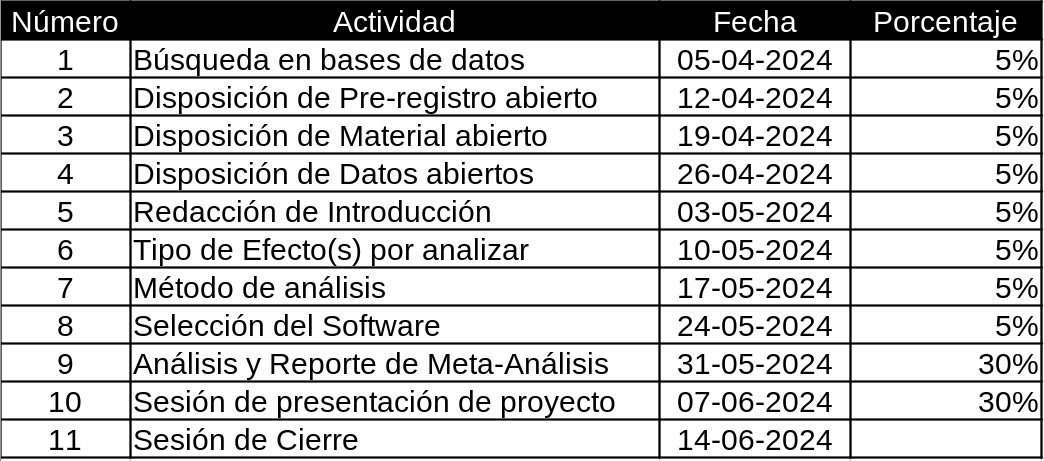
\includegraphics[width=0.7\linewidth]{Notas.png}
\end{figure}
\end{frame}

\begin{frame}{Recomendaciones para el máximo rendimiento}
\begin{itemize}
\item[1.] Observe y aprenda de manera vicaria, aplicando los trucos ilustrados en la clase para cada .
\item[2.] Adopte la tecnología para acelerar su rendimiento (e.g., R, Overleaf, Python, SciSpace Copilot, OSF, GitHub).
\item[3.] Expóngase preferentemente a la literatura sugerida en este curso.
\end{itemize}
\end{frame}

\begin{frame}
\begin{block}{Al finalizar esta clase, usted debe saber:}
\vspace{.2cm}
\begin{itemize}
\item[1] Por qué es fundamental saber buscar en varias bases de datos. 
\vspace{.2cm}
\item[2] Por qué se habla sobre ``Ciencia Abierta'' en relación con los meta-análisis.
\vspace{.2cm}
\item[3] Las herramientas computacionales para la realización de un meta-análisis. 
\end{itemize}    
\end{block}
\end{frame}



\section{¿Por qué y para qué un meta-análisis?}

\begin{frame}{¿Por qué un meta-análisis?}
\centering
\begin{figure}

\includegraphics[width=0.7\linewidth]{Claridad.png}
\end{figure}
Porque su método da como resultado una visión más clara del tema.
\end{frame}

\begin{frame}{¿Para qué un meta-análisis?}
\centering
\begin{figure}

\includegraphics[width=0.3\linewidth]{RoyalSociety.png}
\end{figure}
Para evitar ser influido por autoridades o creencias imperantes de la sociedad. \\
(\textit{Nullius in Verba}).
\end{frame}

\begin{frame}
\begin{columns}
\begin{column}{0.5\textwidth}
John Kapoor (Fundó Insys Therapeutics, la principal productora de fentanilo, un potente opiode liberador del dolor para pacientes crónicos con cáncer. El fentanilo adquirió popularidad debido a que la compañía tenía la práctica de sobornar a médicos profesionales para que actuaran como ``promotores'' del medicamento incluyendo a pacientes sin cáncer. La película \textit{Pain Hustlers} ilustra esta práctica).\\
\end{column}
\begin{column}{0.5\textwidth}
\begin{figure}

\includegraphics[width=.5\textwidth]{Pain.png}
\end{figure}   
\end{column}
\end{columns}
\end{frame}

\begin{frame}
\begin{columns}
\begin{column}{0.5\textwidth}
Francesca Gino (Profesora de la escuela de negocios de Harvard University está acusada de fabricar datos en cuatro de sus artículos, incluyendo uno publicado en 2012 por la prestigiosa revista PNAS).\\
\end{column}
\begin{column}{0.5\textwidth}
\begin{figure}

\includegraphics[width=.7\textwidth]{Gino.png}
\end{figure}   
\end{column}
\end{columns}
\end{frame}

\begin{frame}
\centering
\begin{figure}

\includegraphics[width=0.65\linewidth]{Moreau.png}
\end{figure}
Hacer un meta-análisis implica seguir tres pautas: 1) pre-registro, 2) material abierto y 3) datos abiertos \parencite{Moreau2022}
\end{frame}

\begin{frame}
\begin{figure}
\centering
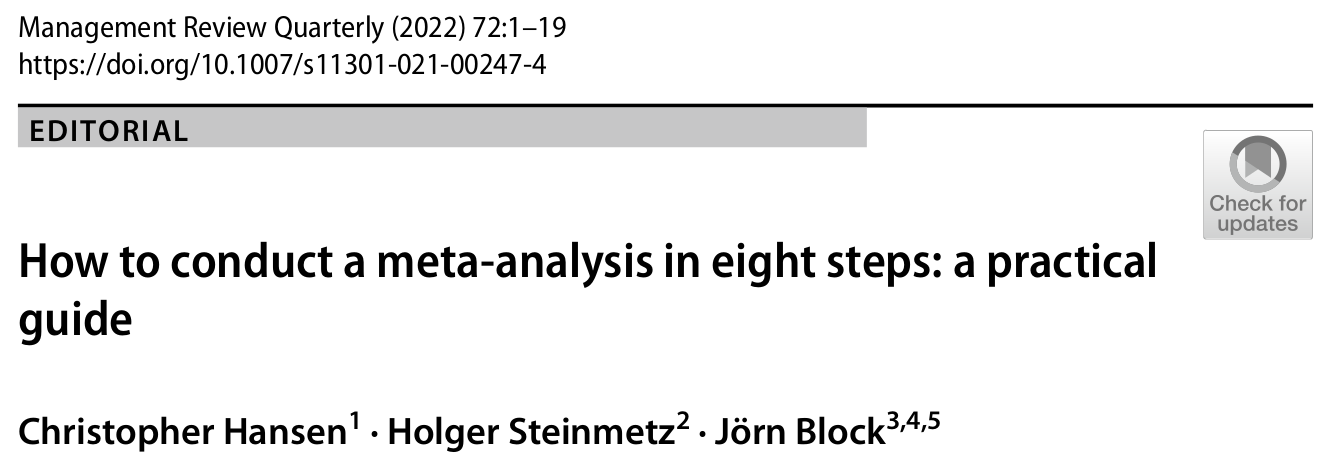
\includegraphics[width=0.9\linewidth]{Hansen.png}
\end{figure}
Para \textcite{Hansen2022}, cualquier meta-análisis puede hacerse en ocho pasos.
\end{frame}

\begin{frame}
\begin{figure}
\centering

\includegraphics[width=0.5\linewidth]{AR.png}
\end{figure}
\textcite{Siddaway2019} brinda un panorama amplio en el que los meta-análisis se consideran un tipo de revisión sistemática. 
\end{frame}

\section{Actividad Evaluada Número 1}
\begin{frame}{Actividad Evaluada Número 1}
En 20 minutos, cada uno de ustedes va a buscar y descargar un artículo (texto completo en pdf) que esté publicado en alguna base de datos indexada (preferentemente en Scopus, PubMed, o Web of Science).\\
\vspace{1cm}
Haremos una sesión comparativa para observar ``la anatomía de un meta-análisis'' a partir de un tema seleccionado según su preferencia.
\end{frame}

\begin{frame}{Actividad de Aprendizaje}
\centering
¿Cómo usar estos recursos para revisión de literatura?
\begin{figure}

\includegraphics[width=0.9\linewidth]{BasesDatos.png}
\end{figure}
¿Hay diferencias entre ellos?
\end{frame}

\begin{frame}{Condiciones para la Entrega}
\begin{itemize}
\item[1.] La fecha límite para la entrega de esta actividad es el 12-04-2024.
\item[2.] La entrega antes de la fecha límite conlleva a un bono automático del 1\% sobre la calificación obtenida para el proyecto.
\item[3.] La entrega debe incluir el enlace al repositorio abierto en OSF o GitHub para garantizar la transparencia de su avance en el proyecto. 
\item[4.] La entrega formal es una presentación donde se comuniquen los criterios de inclusión y exclusión para la muestra de artículos a analizar (siguiendo el ejemplo del artículo texto completo conseguido para la actividad evaluada número 1). 
\end{itemize}
\end{frame}



\begin{frame}[allowframebreaks]{Referencias}
\printbibliography[heading=none]
\end{frame}

\end{document}